\documentclass[7pt]{article}

\usepackage{amsmath}
\usepackage{graphicx}
\usepackage{caption}
\usepackage[landscape]{geometry}
\usepackage{multicol}
\usepackage{amssymb}

\usepackage{geometry}
\geometry{
 a4paper,
 total={285mm,185mm},
 left=10mm,
 top=10mm,
}

\setcounter{section}{5}
\setlength\columnseprule{0.5pt}
\setlength{\parindent}{0pt}
\graphicspath{ {images/} }

\begin{document}
\begin{multicols*}{3}

\section{Relativit{\"a}t}

\subsection{Relativbewegung}

Beobachter, die sich relativ zueinander bewegen, messen verschiedene Geschwindigkeiten und Beschleunigungen:
\begin{equation*}
\begin{array}{ll}
	\underbrace{v(t)}_\text{relativ zu O} = \frac{dR(t)}{dt} + \underbrace{v'(t)}_\text{relativ zu O'} \\
	\underbrace{a(t)}_\text{relativ zu O} = \frac{d^2R(t)}{dt^2} + \underbrace{a'(t)}_\text{relativ zu O'}
\end{array}
\end{equation*}

\subsection{Scheinkr{\"a}fte}

Ein \textbf{Inertialsystem} ist ein Bezugssystem, in dem die Newtonschen Gesetze gelten. Es ist \emph{nicht beschleunigt}. \\

Die \textbf{Zentrifugalkraft} ist eine fiktive, nach aussen gerichtete Kraft:
\begin{equation*}
	F_{ZF} = m(r'\omega^2)e_r
\end{equation*}

Die \textbf{Corioliskraft} wirkt senkrecht zur radialen Geschwindigkeit:
\begin{equation*}
	F_C = m(2v'\omega)e_\varphi
\end{equation*}

\emph{Hinweis:} Ein Bezugssystem, das feste Koordinaten relativ zur Erdoberfl{\"a}che hat ist kein Inertialsystem, da die Erde sich dreht/beschleunigt ist.

\subsection{Transformationen}

\subsubsection{Ereignis}

\begin{equation*}
	x^\mu \equiv (ct, x, y, z)
\end{equation*}
wobei das Produkt $ct$ die Lichtgeschwindigkeit $[\frac{m}{s}]$ mal die Zeit $[s]$ ist.

\subsubsection{Galileitransformation}

Wir betrachten zwei Beobachter $O$ und $O'$, die sich relativ zueinander mit \emph{konstanter Geschwindigkeit} bewegen.

\begin{center}
	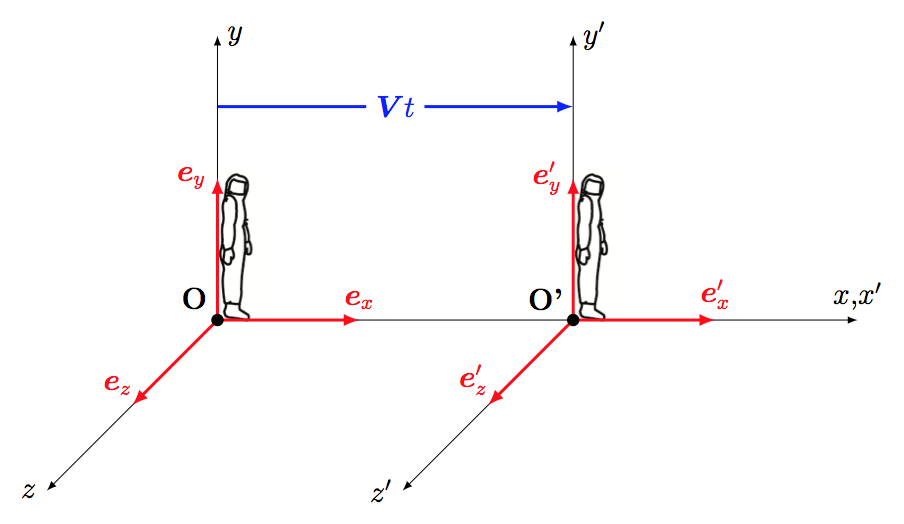
\includegraphics[width=200pt]{images/galileitransformation}
\end{center}

Bewegt sich der Beobachter $O'$ in positive Richtung der x-Achse des Bezugssystems $O$, so ist die Transformation gleich
\begin{equation*}
	\left\{
		\begin{array}{ll}
			ct' = ct \\
        	x' = x - \beta ct\\
            y' = y \\
            z' = z \\
		\end{array}
	\right.
	\text{von O nach O'}
\end{equation*}
\begin{equation*}
	\left\{
		\begin{array}{ll}
			ct = ct' \\
        	x = x' + \beta ct\\
            y = y' \\
            z = z' \\
		\end{array}
	\right.
	\text{von O' nach O}
\end{equation*}
wobei der \textbf{Geschwindigkeitsparameter $\beta$} $= \frac{V}{c}$ ist. 

\subsubsection{Lorentz-Transformation}

Der \textbf{Lorentz-Faktor} ist gleich
\begin{equation*}
	\gamma = \frac{1}{\sqrt{1-\beta^2}}
\end{equation*}

Dann ist die Transformation gleich
\begin{equation*}
		\left\{
		\begin{array}{ll}
			ct' = \gamma(ct - \beta x) \\
        	x' = \gamma(x - \beta ct) \\
            y' = y \\
            z' = z \\
		\end{array}
	\right.
	\text{von O nach O'}
\end{equation*}
\begin{equation*}
		\left\{
		\begin{array}{ll}
			ct = \gamma(ct' + \beta x') \\
        	x = \gamma(x' + \beta ct') \\
            y = y' \\
            z = z' \\
		\end{array}
	\right.
	\text{von O' nach O}
\end{equation*}

\subsubsection{Geschwindigkeitstransformation}

Der \textbf{Geschwindigkeitsvektor $u$} bez{\"u}glich $O$ kann wie folgt berechnet werden

\begin{equation*}
	\begin{array}{ll}
		u_x = \frac{u'_x + V}{1 + \frac{\beta}{c}u'_x} \\
		u_y = \frac{u'_y}{\gamma(1+\frac{\beta}{c}u'_x)}
	\end{array}
\end{equation*}

\subsection{Relativit{\"a}tstheorie}

\subsubsection{Raumzeit-Intervall}

R{\"a}umliche und zeitliche Entfernungen sin in verschiedenen Bezugssystemen unterschiedlich. Nur das \textbf{Raumzeit-Intervall $\Delta s$} ist gleich f{\"u}r alle Beobachter.
\begin{equation*}
	\Delta s^2 = \underbrace{(c\Delta t)^2}_{\substack{\text{zeitliche}\\ \text{Entfernung}}} - \underbrace{\Delta r^2}_{\substack{\text{r{\"a}umliche}\\ \text{Entfernung}}}
\end{equation*}

\subsubsection{Zeitdilatation}

Das in einem bewegten Bezugssystem gemessene Zeitintervall ist immer um den Faktor $\gamma$ gr{\"o}sser als das Eigenzeitintervall:
\begin{equation*}
	\underbrace{\Delta t'}_{\substack{\text{bez{\"u}glich $O'$}\\ \text{gemessene Zeit}}}  =  \underbrace{\gamma \cdot \Delta\tau}_{\substack{\text{bez{\"u}glich $O$}\\ \text{gemessene Zeit}}}
\end{equation*}
wobei $\Delta\tau$ das Eigenzeitintervall ist (Zeit im Ruhesystem gemessen). \\

Daraus folgt, dass Vorg{\"a}nge l{\"a}nger zu dauern scheinen, wenn sie in einem System ablaufen, das sich relativ zum Beobachter bewegt.

\subsubsection{L{\"a}ngenkontraktion}

Die r{\"a}umliche Entfernung zwischen zwei Punkten erscheint geringer, wenn sich der Beobachter relativ zu diesen Punkten bewegt, als wenn er relativ zu ihnen ruht:
\begin{equation*}
	\underbrace{\Delta x'}_{\substack{\text{bez{\"u}glich $O'$}\\ \text{gemessene L{\"a}nge}}}  =  \underbrace{\frac{\Delta\lambda}{\gamma}}_{\substack{\text{bez{\"u}glich $O$}\\ \text{gemessene L{\"a}nge}}}
\end{equation*}
wobei $\Delta\lambda$ die Eigenl{\"a}nge ist (L{\"a}nge im Ruhesystem gemessen).\\
1 electronVolt = $1.6*10^{-19}J$

\end{multicols*}
\end{document}